\def\VCDate{2016/03/18}\def\VCVersion{(Current)}
\documentclass{article}
\usepackage[screen]{geometry}
\usepackage[hypcap]{caption}
\usepackage{ProofPower, verbatim, graphicx, color, amsmath, amssymb, hyperref, multicol}
\begin{document}
\underscoreoff

\title{CS118 Lab:1}
\author{Saw Thinkar Nay Htoo}
\maketitle

\section*{Model the store (memory)}
To model the way memory changes as a computation progresses. We will use some global variables, some local variables, and some registers. Use a diagrams to 
illustrate the code as it progresses, showing how each instruction changes the state. 

\section*{Analysis}
Create some variables of each type. Use the debugger to find the actual memory addresses of each.
Use IPE to label a diagram with those addresses and values. Make new diagram for each statement/instruction that changes the store. 
e.g. A program that does a summation of several numbers (without control structures such as loops and if statements. Let x = 2, y = 3, and z = 4 in r = x + y + z is an example.

\section*{Tools}
Photoshop is used instead of IPE, with similiar concept of usage which is using the separate layers so that images of the changes can be made easily.
\clearpage
\clearpage

\section*{My very own concept of this lab.}
\textbf{All these weeks, I have been trying to figure out almost everything concerning with assembly language programming. Now I feel like I reached up to a point where I can explain some of the contents back with my own understanding of what I have observed. So this lab will not be perfect, and might a bit different from what the professor expects to see although I included all the lab requirement. However, I will still keep improving with this throughout the whole semester. I will try my best to reference and cite all the contents I have read, found out, analyzed and refered.}
\clearpage

This is the SML code of the example algorithm which will be later be converted to C then to ASM. 
\section*{Prototype SML code}
\begin{GFT}{SML}
\+val x = 2;\\
\+val y = 3;\\
\+val z = 4;\\
\+val w = 6;\\
\+val s = 5;\\
\+val r = x + y + z;\\
\+val r = r + s;\\
\+val r = r + w;\\
\end{GFT}
These are not assigning to the store (SML does not support assignment like this)
It is more like symbolic constants putting the value in a symbol table. 
\section*{Output from SML code}
\verbatiminput{result}
\clearpage


\section*{C code implementation of the SML code}
\begin{minipage}{4cm}
\begin{GFT}{Text written to file lab2.c}
\+\#include <stdio.h>\\
\+\#define x 2 		\\
\+const int y = 3;	\\
\+int t; 			\\
\+int w =6; 		\\
\+int main()\\
\+\{\\
\+  register int z = 4;	\\
\+  int r = x + y + z;	\\
\+  static int s =5; 	\\
\+  r +=s;\\
\+  r += w;\\
\+  printf("r=\%i\Backslash{}n",r);	\\
\+  return 0;		\\
\+\}\\
\end{GFT}
\end{minipage}
\begin{minipage}{10cm}
"C code explanation"\\
:C library \\
:symbolic constant. int x = 2; \\
:global named (typed) constant\\
:(int t;) will be stored in bss segment (Uninitialized data segment)\\
:data segment\\
:\\
:int main() is stored in .text segment\\
:\\
:register \\
:Being operated on the stack. Now r result is x = 2+3+4 =9 \\
:static local in data segment \\
:In this step, the value of s is added to r. r + 5 = 9+5 = 14 \\
:In this step, the value of w is added to r. r + 6 = 14+6 = 20 \\
:This is to print out the last r value which is 20. Thus the output is "r=20".\\
:return statement\\	
:\\
\end{minipage}


The output when running this C program in the console is:
\verbatiminput{cresult}
\clearpage


In the debugger, the memory addresses of the 4 variables are:
\begin{description}
\item[x:] is stored in the instruction (add 83 c0 02) at location 0x8048417
\item[y:] 0x80484f0 (rodata)
\item[t:] 0x8049710 (bss)
\item[w:] 0x8049704 (data)
\item[z:] ebx register
\item[r:] 0xbffff61c r is on the stack 0xc bytes below ebp (changed from 0xbffff61e to 0xbffff61c)
\item[s:] 0x8049708 (uninitialized small data)
\end{description}
The stack frame uses register ebp ( base pointer) and esp (stack pointer) to find the values related to one function call. The stack pointer points to the most recent value pushed onto the stack. The base pointer points to a mid-point in the frame with the functon parameters above it, and the local variables below it. ebp is at the location oxbffff628. 

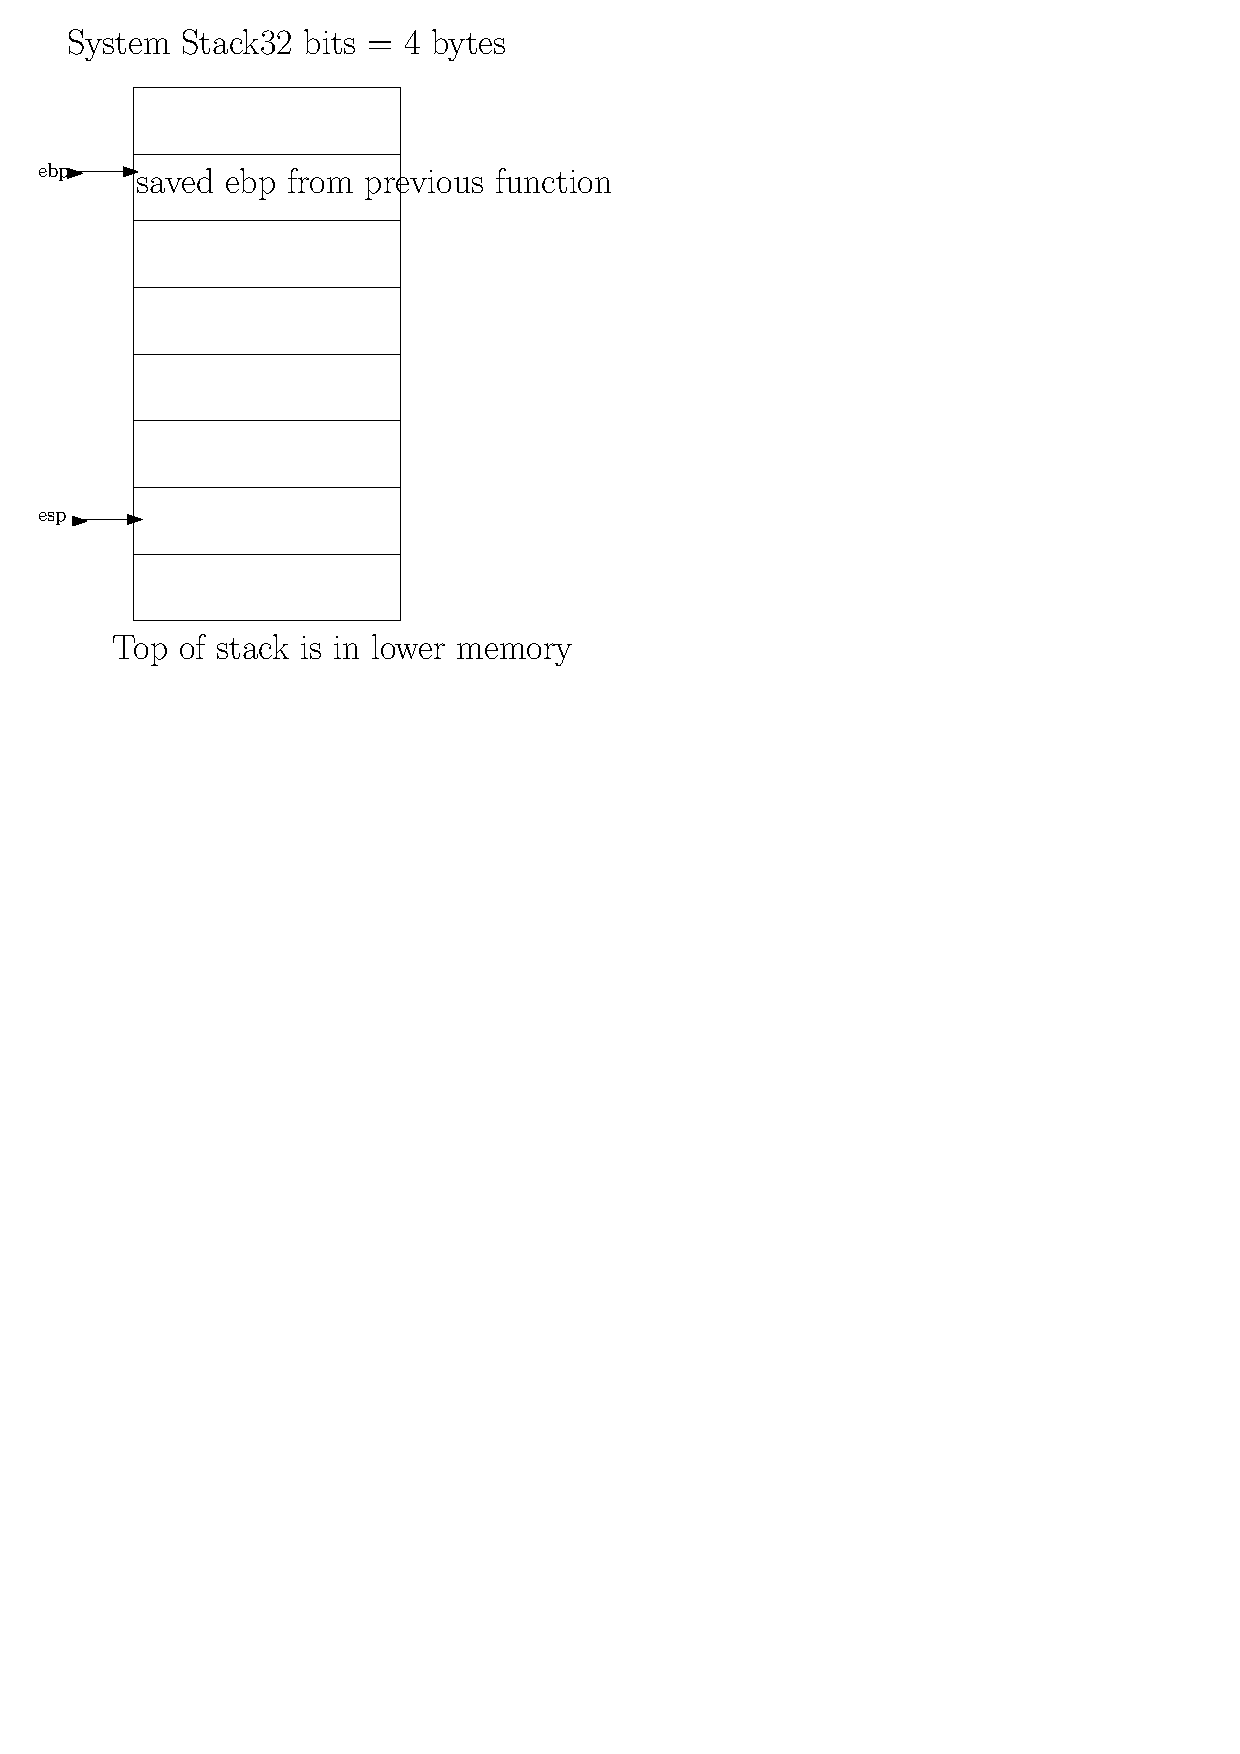
\includegraphics{stackframe.pdf}

\section*{Memory Segments}
Recreated Concept of Memory Segments from this \href{http://goo.gl/SbQhnH}{blog}.\\
\begin{minipage}{11cm}
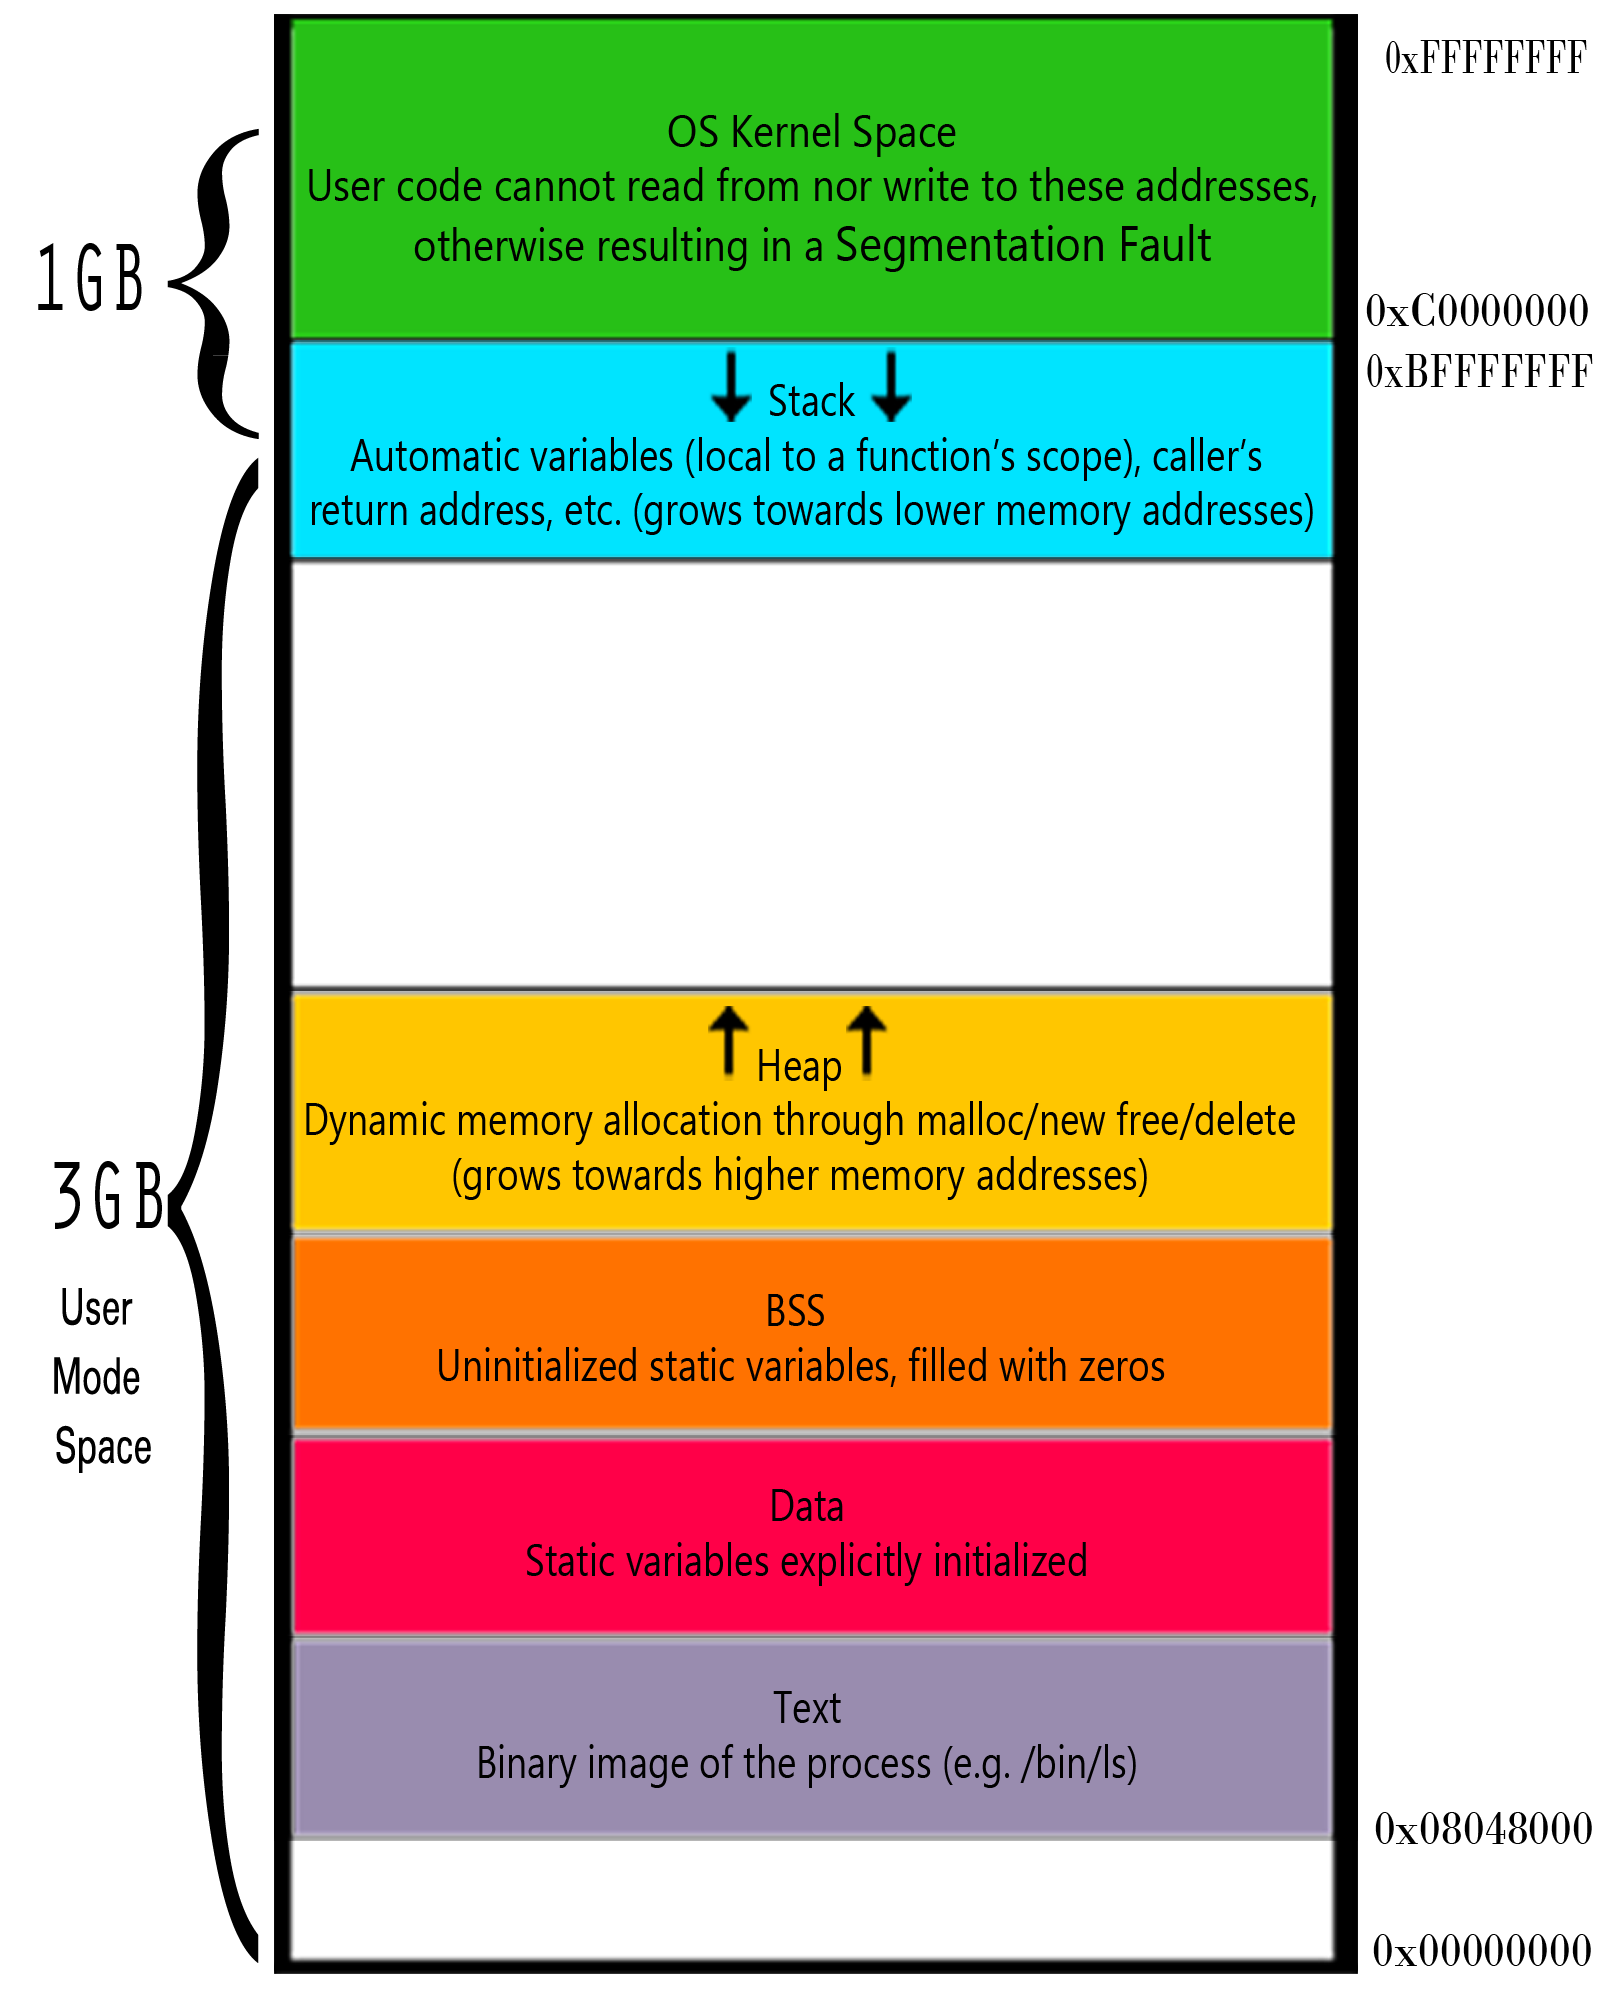
\includegraphics[scale=0.5]{memory.PNG}
\end{minipage}
\begin{minipage}{7cm}
Below addresses information are obtained from the \hyperlink{st}{Symbol Table} of the objdump result of my ASM program.
\begin{itemize}
\item
Stack\\
\item
Heap\\
\item
BSS\\
From 080496c0 \\
to 080496c8
\item
Data\\
From 080496b0 \\
to 080496c0
\item
Text\\
From 08048300 \\
to 08048300 \\
Though I couldn't find the end address of Text in the symbol table in terminal, it can be obtained from the given memory segment diagram. 
\end{itemize}
\end{minipage}
\clearpage

\section*{Overall explanation of the segments}
\begin{itemize}
\item
Text\\
This is the code segment with executable instructions of the ASM program. Usually placed below Stack or Heap in order to prevent overflows from overwriting this segment. Most importantly, the text segment is often Read-only/Execute to prevent from being modifited its instructions accidentally.
\item
Data\\
This segment contains global and static variables which are initialized by the programmer. Furthermore, it can be classified into initialized Read-only(RoData) and initialized Read-Write sections. 
\item
BSS\\
(Block Started by Symbol) This segment is also known as Uninitialized data segment. This is a Read-Write segment and usually starts after data segment and have all global and static variables that are initialized to zero or are not initialized. For example, int i.
\item
Stack\\
Stack usuallys located in the higher memory addresses right below the OS kernel space. On the standard x86, it grows downwards to lower addresses, while Heap grows up. (In some architectures, they may grow in different directions. The set of values pushed for one function call is named a stack frame.
\item
Heap\\
Heal is the segment where dynamic memory allocation usually takes place. It is managed by malloc/new and free/delete to adjust its size.
\end{itemize}
\clearpage


\section*{Symbol Table}
\hypertarget{st}{Symbol Table} \\
In my opinion, it is definitely important to be able to handle well with symbol table while using GDB. \href{http://goo.gl/ygJ29f}{Click here} to get the simple idea of what a symbol table is. In the symbol table, size, address, segments and other important information are shown clearly in each catagory. \\
terminal command to see the Symbol Table of the labasm file: \\
objdump -x labasm \\
\section*{Symbol Table result in terminal}
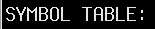
\includegraphics[scale =0.5]{st.png} \\
Start and end address of BSS segment is shown below. \\
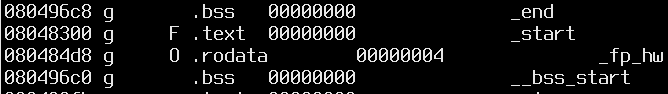
\includegraphics[scale =0.5]{bssadd.png} \\
Start and end address of DATA segment is shown below. \\
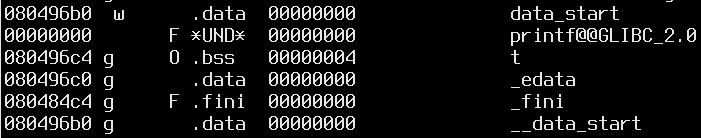
\includegraphics[scale =0.5]{dataadd.png} \\
\clearpage

\section*{Translation of C code to ASM code}
\begin{itemize}
\item \verb|#define x 2| 	$\rightarrow$ .equ x,2
\item const int y = 3 	$\rightarrow$ .section .rodata y: .long a
\item int t;		$\rightarrow$ .bss .comm t,4
\item int w =6;		$\rightarrow$ .data w: .long 6
\end{itemize}
\begin{GFT}{Text written to file lab2.s}
\+.equ x,2\\
\+.section .rodata\\
\+y: .long 3\\
\+.bss\\
\+.comm t,4\\
\+.data\\
\+w: .long 6\\
\end{GFT}
\clearpage




\begin{itemize}
\item int main() $\rightarrow$ .text .globl main main:
\item \verb|printf("r=%in",r");| $\rightarrow$
 \begin{itemize}
 \item .section .rodata msg: .string \verb|"r=%i\n"|
 \item .text call printf
 \end{itemize}
\end{itemize}
\begin{GFT}{Text appended to file lab2.s}
\+.text\\
\+.globl main\\
\+main:\\
\+ .section .rodata\\
\+ msg: .string "r=\%i\Backslash{}n"\\
\+.data\\
\+s:.long 5\\
\+ .text\\
\end{GFT}
\clearpage





\begin{itemize}
\item \verb|int r = x+y+z| 	 
\end{itemize}
Below is the ASM code for above calculation. 4 bytes is substracted from the stack where esp is pointing at. Then the empty space is filled with x. Then y is moved to eax. Then the value of eax is add to the value of the address where esp is pointing, giving out the result of 5. In next step, 4 is moved to ebx and it is add to the value of the address where esp is pointing which is 5, giving out the result of 9.
\begin{GFT}{Text appended to file lab2.s}
\+sub \$4,\%esp \# make room on stack for local variable\\
\+movl \$x,(\%esp) \#derefrence the point just like asteroid in CPP.\\
\+mov y,\%eax\\
\+add \%eax,(\%esp)\\
\+mov (\%esp),\%ebx \#ebx now has 5\\
\+mov \$4,\%ebx\\
\+add \%ebx,(\%esp)\\
\+mov (\%esp),\%edx \#edx now has 9\\
\end{GFT}
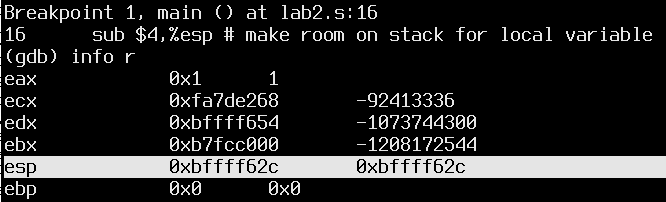
\includegraphics[scale = 0.6]{infor1.png} \\
This is the initial values and addresses of the registers before making changes.
\clearpage

\verb|sub $4,%esp| \\
After above line of code, 4 bytes substracted from the stack. Initial esp address 0xbffff62c, then becomes 0xbffff628. \\
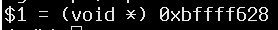
\includegraphics[scale = 0.6]{pesp1.png} \\
\noindent{\color{red}\rule{\linewidth}{0.5mm}}

\verb|mov y,%eax| \\
After above line of code, eax now holds the value "3". \\
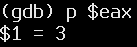
\includegraphics[scale = 0.6]{eax1.png} \\
\noindent{\color{red}\rule{\linewidth}{0.5mm}}

\verb|add %eax,(%esp)| \\
\verb|mov(%esp),%ebx | \\
After the addition is operated, the value, pointed by esp, is moved to ebx in order to print out the result. \\
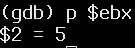
\includegraphics[scale = 0.6]{ebx1.png} \\
\noindent{\color{red}\rule{\linewidth}{0.5mm}}

\verb|mov $4,%ebx| \\
Now a new value is moved into ebx. \\
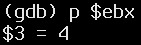
\includegraphics[scale = 0.6]{ebx2.png} \\
\noindent{\color{red}\rule{\linewidth}{0.5mm}}
\clearpage

\verb|add %ebx,(%esp)| \\
\verb|mov (%esp),%edx| \\
After the addition is operated, the value, pointed by esp, is moved to edx in order to print out the result. \\
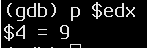
\includegraphics[scale = 0.6]{edx1.png} \\
\noindent{\color{red}\rule{\linewidth}{0.5mm}}

\begin{itemize}
\item \verb|int r += s;| 	 
\end{itemize}
\begin{GFT}{Text appended to file lab2.s}
\+mov s,\%ebx\\
\+add \%ebx,(\%esp)\\
\+mov (\%esp),\%edx \#edx now has 14\\
\+\\
\end{GFT}
\verb|mov s,%ebx| \\
\verb|add %ebx,(%esp)| \\
\verb|mov (%esp),%edx| \\
After the addition is operated (s + 9), the value, pointed by esp, is moved to edx in order to print out the result (14). \\
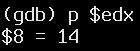
\includegraphics[scale = 0.6]{edx3.png} \\
\noindent{\color{red}\rule{\linewidth}{0.5mm}}
\begin{itemize}
\item \verb|int r += w;| 	 
\end{itemize}
\begin{GFT}{Text appended to file lab2.s}
\+mov w,\%ebx\\
\+add \%ebx,(\%esp)\\
\+mov (\%esp),\%edx \#edx now has 20\\
\end{GFT}
\verb|mov w,%ebx| \\
\verb|add %ebx,(%esp)| \\
\verb|mov (%esp),%edx| \\
After the addition is operated (w + 14), the value, pointed by esp, is moved to edx in order to print out the result (20). \\
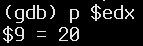
\includegraphics[scale = 0.6]{edx4.png} \\
\noindent{\color{red}\rule{\linewidth}{0.5mm}}
\clearpage 


\begin{itemize}
\item Now print the value of r	 
\end{itemize}
\begin{GFT}{Text appended to file lab2.s}
\+ push (\%esp)\\
\+ push \$msg\\
\+ call printf\\
\+ add \$8, \%esp \#clean up stack parameters\\
\+ add \$4, \%esp \#clean up  local parameters\\
\+ ret\\
\end{GFT}


\verb|add $8, %esp| \\
\verb|add $4, %esp| \\
\verb|ret| \\
In this case, the print value of esp should be ...28. I don't what happened during the process. \\
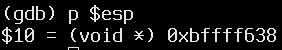
\includegraphics[scale = 0.6]{pesp2.png} \\
\noindent{\color{red}\rule{\linewidth}{0.5mm}}
After \\
\verb|push (%esp)| \\
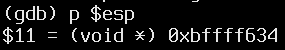
\includegraphics[scale = 0.6]{pesp3.png} \\
\noindent{\color{red}\rule{\linewidth}{0.5mm}}
After \\
\verb|push $msg| \\
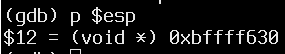
\includegraphics[scale = 0.6]{pesp4.png} \\
\noindent{\color{red}\rule{\linewidth}{0.5mm}}
After
\verb|call printf| \\ 
The address goes back to the initial value after cleaning up the stack and local parameters, by adding 8 and 4 to the addresses. \\
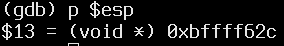
\includegraphics[scale = 0.6]{pesp5.png} \\
\noindent{\color{red}\rule{\linewidth}{0.5mm}}

\section*{LABASM OUTPUT}
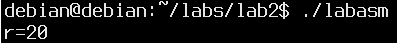
\includegraphics[scale = 0.6]{labasmout.png} \\

\clearpage
\section*{Shell scripts to make processing easier}
This shell script is used to make extracting and processing the source code easier. The -g option to the gcc compiler adds debugging symbols so we can refer to variables even though they are not normally stored in the object code. 

\begin{GFT}{Text written to file labcode.sh}
\+docsml lab2.doc\\
\+gcc -Wall -o labc lab2.c\\
\+gcc -Wall -o labasm lab2.s\\
\+\\
\end{GFT}
\begin{GFT}{Text written to file labdbg.sh}
\+docsml lab2.doc\\
\+gcc -Wall -g -o labc lab2.c\\
\+gcc -Wall -g -o labasm lab2.s\\
\+\\
\end{GFT}
\begin{GFT}{Text written to file labdoc.sh}
\+doctex lab2.doc\\
\+pptexenv /home/debian/texfot.pl pdflatex lab2.tex\\
\end{GFT}
\begin{GFT}{Bourne Shell}
\+chmod 755 labcode.sh \\
\+chmod 755 labdoc.sh\\
\+chmod 755 labdbg.sh\\
\+poly < lab2.sml > result\\
\+./labc > cresult\\
\+\\
\end{GFT}
\begin{GFT}{Text written to file dbg\_cmds}
\+b main\\
\+r\\
\+info r\\
\end{GFT}
warning messgae: \href{http://web.stanford.edu/class/cs107/guide_gdb.html}{"Source file is more recent than executable."}
\begin{GFT}{Bourne Shell}
\+touch labc \#to get rid of the warning message mentioned above.\\
\+gdb --quiet -x dbg\_cmds labc | grep -v 'Ignore\Backslash{}|Quit'| tee labc.log\\
\+\\
\end{GFT}
\clearpage
...below is the output of automated script for GDB:
\verbatiminput{labc.log}

\end{document}
